% $Id: results.tex$
% !TEX root = main.tex

\chapter{Results}
\subsection{Carla}
On CARLA experiment it was possible to train up to 32.000 iterations which took around 32 hours of training, however, due to technical difficulties related with the hardware, and the model being computationally expensive, it was not possible to train any further, the simulator requires 6Gb of video memory out of the 8 that comes with the Nvidia 4060 ti, which only leaves 2Gb of memory to train. Even though as shown in figure the reward seems to go up, the variance through episodes is too high and the agent doesn't take any action that from a human perspective is ideal. From this point, it was decided to not move forward this simulator.

\begin{figure}[h]
    \centering
    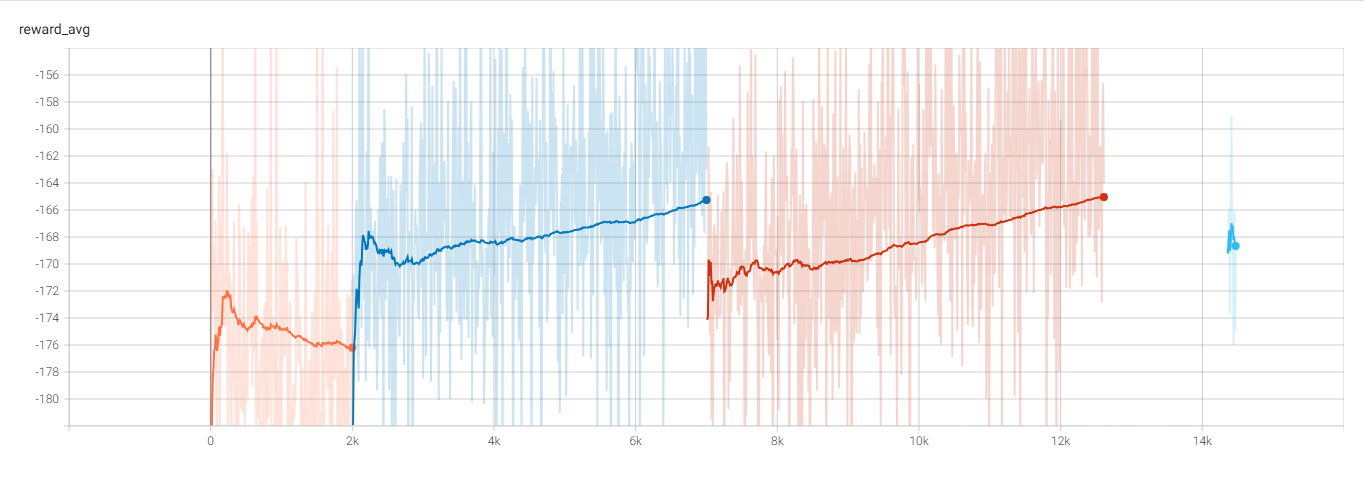
\includegraphics[width=0.8\textwidth]{./figures/CARLA_ddpg_14k_iters.png}
    \caption{CARLA TD3 Cybertruck train log, 14000 iterations.}
\end{figure}

\subsection{Gazebo ROS}
All agents were trained until they reach the final goal 10 times in a row without crashing. The right experiment took around 6 hours to train, maximum the average reward was 3150 as shown in \fref{fig:gazebo_right_avg}.

\begin{figure}[h]
    \centering
    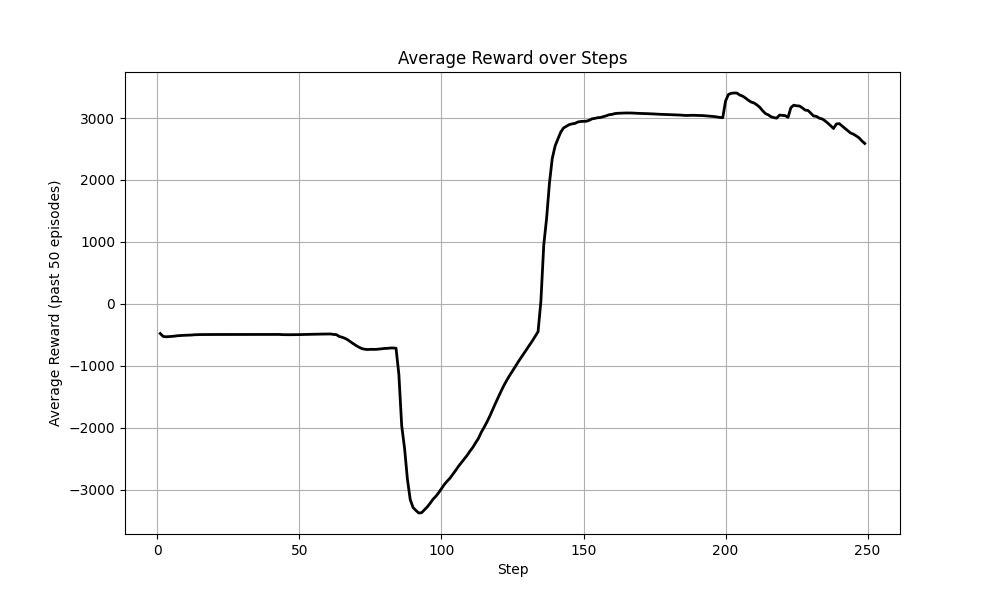
\includegraphics[width=0.65\textwidth]{./figures/rigth_no_tl_avg_reward_past_50_episodes.png}
    \caption{Gazebo ROS right agent train log, Reward gained per episode.} 
    \label{fig:gazebo_right_avg} 
\end{figure}

The left experiment took around 8 hours to train, the maximum average reward was 3108 as shown in \fref{fig:gazebo_left_avg}. Even though this experiments took less steps to train, the time it took was longer, this is because the environment ends a step only when there is a crash, so it's episodes could be longer than the right agent.

\begin{figure}[h]
    \centering
    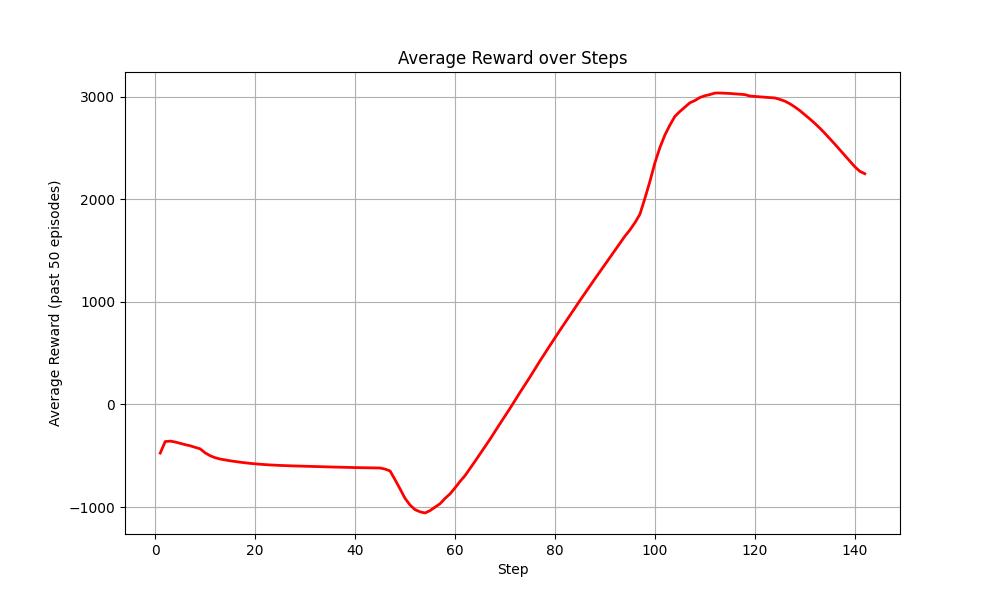
\includegraphics[width=0.65\textwidth]{./figures/left_no_tl_avg_reward_past_50_episodes.png}
    \caption{Gazebo ROS left agent train log, Reward gained per episode.} 
    \label{fig:gazebo_left_avg}
\end{figure}

We can see in \fref{fig:gazebo_right_avg} and \fref{fig:gazebo_left_avg} a tendency of the reward to go down on the first episodes before it starts to go up, this is a common behavior in  TD3\cite{TD3} and DDPG\cite{ddpg} algorithms.

Once we have the expert agents trained, we are going to use the right expert agent to keep training in the other paradigm without expert demonstration learning to have a baseline to compare the results. The agent took around 8 hours to train from the base expert and the maximum reward it achieved was 3150 and the full training can be seen in \fref{fig:gazebo_right_left_avg}.

\begin{figure}[h]
    \centering
    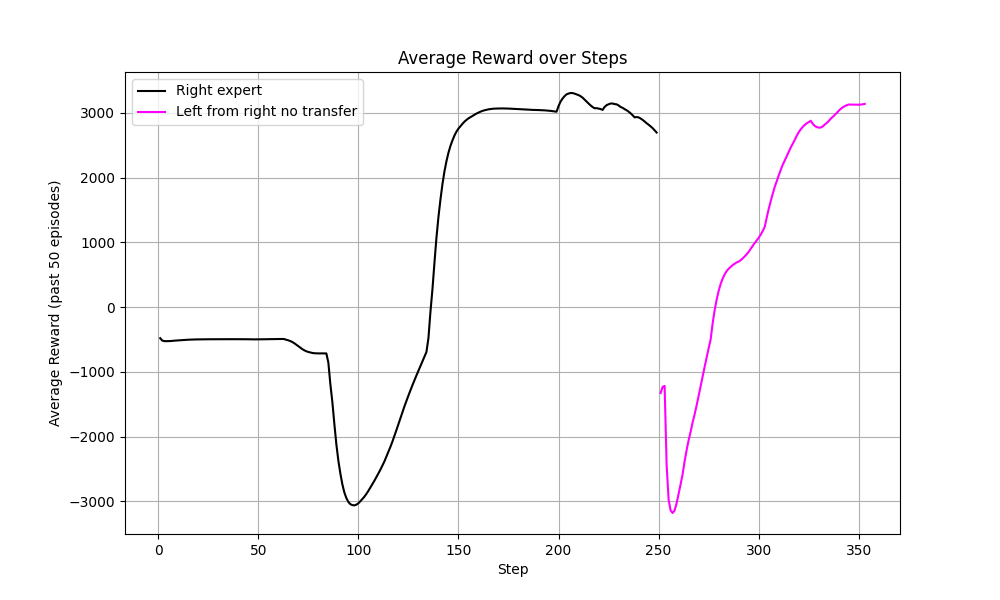
\includegraphics[width=0.65\textwidth]{./figures/right_left_no_transfer.png}
    \caption{Gazebo ROS left agent train log,Reward gained per episode.} 
    \label{fig:gazebo_right_left_avg}
\end{figure}

In \fref{fig:gazebo_right_left_avg} we can see the transition between the expert agent and its continuation to the other side, We can see here that it took less steps than training the agent from 0. Notice how the reward goes down again at the beginning of both training, once again, this is a characteristic of the TD3 algorithm.

The next agent was trained from the expert right agent on the left environment, this time using \fref{eq: pre train gradient pi} and \fref{eq: pre train gradient Q} as part of the training process, this agent took around 1.6 hours to train and the maximum reward it achieved was 3150, the full training can be seen in \fref{fig:gazebo_right_left_transfer}.

\begin{figure}[h]
    \centering
    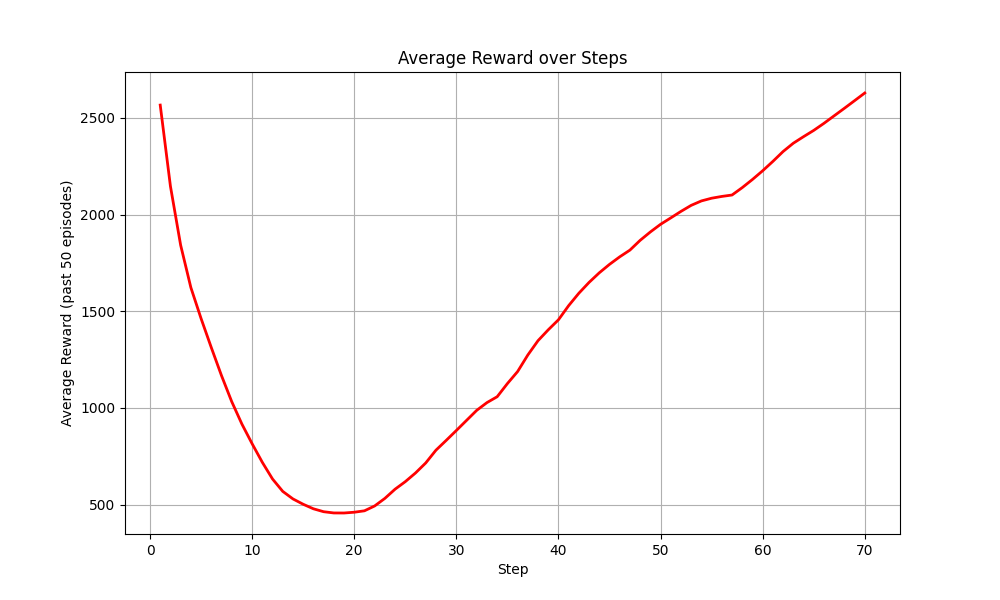
\includegraphics[width=0.65\textwidth]{./figures/tl_right_expert_left_environment.png}
    \caption{Gazebo ROS transfer learning agent train log.} 
    \label{fig:gazebo_right_left_transfer}
\end{figure}

We can put these 3 results together, the right left agent, the left right agent that learned from the right expert agent and the left agent that learned with transfer learning .

\begin{figure}[h]
    \centering
    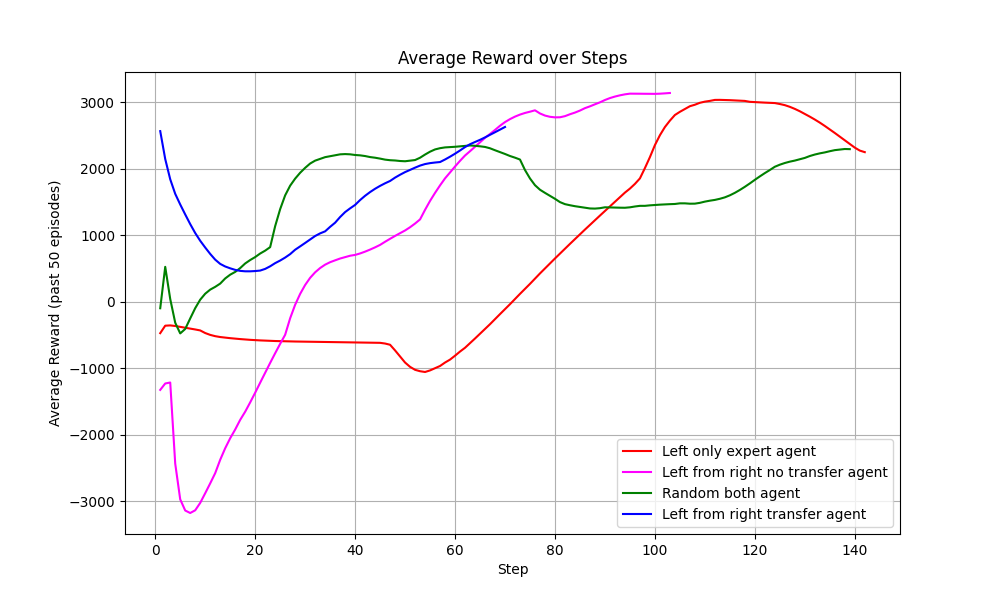
\includegraphics[width=0.68\textwidth]{figures/comparison_1.png}
    \caption{Gazebo ROS comparison of the 3 agents.} 
    \label{fig:gazebo_transfer_learning_comparison}
\end{figure}

The data from the left agent that learned from the right agent but did not use transfer learning was transposed so it's steps start from 0 for the purpose of the comparison. We can see in \fref{fig:gazebo_right_left_transfer} that the agent was able to learn the new environment and achieve the same reward as the expert in less time and within less episodes, this is a clear indicator that the agent was able to transfer the knowledge from the right expert agent to the left environment even though the average reward is lower than the other agents, this may be caused because there was less experiments but we clearly can see how it learned faster than the other agents.

In terms of time there is also a clear difference as shown in , the agent that learned with transfer learning took 1.6 hours to train which is less than the 8 hours that the agent that learned from scratch took, this is a clear indicator of how transfer learning can help to reduce the training time and the number of episodes needed to learn a new environment. 

\begin{figure}[h]
   \centering
   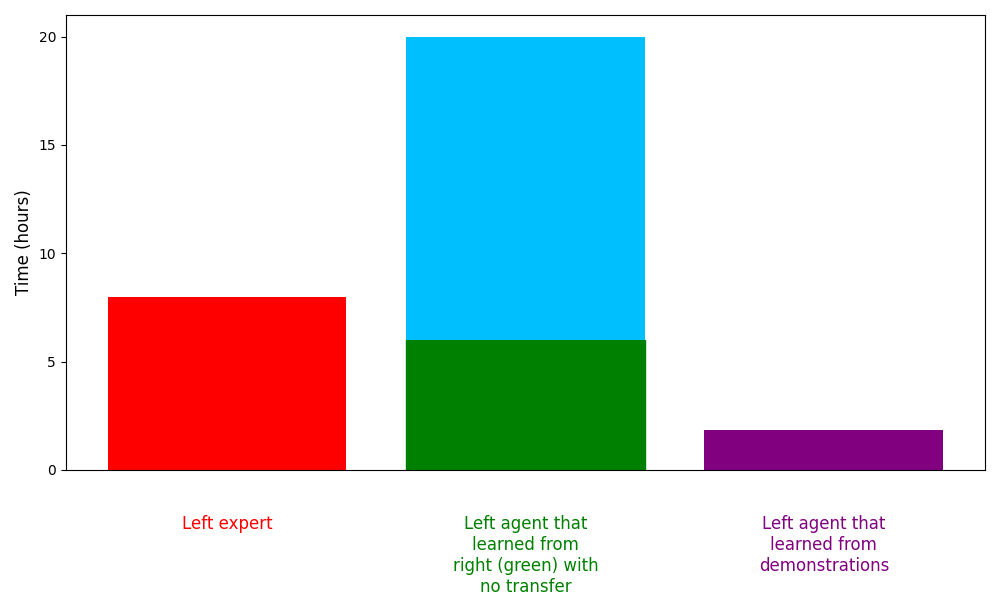
\includegraphics[width=0.6\textwidth]{figures/time_comparison_1.png}
   \caption{Gazebo ROS comparison of the 3 agents in terms of time.} 
\end{figure}